\section{Integración de la no holonomía}
\setlength{\columnseprule}{0pt}
\twocolumn
\subsection{Construcción del error}
De acuerdo con Ramírez y Zeghloul \cite{ramirez2001control} la configuración del robot es:

{\small$\mathbf{q} = \begin{bmatrix} x & y & \theta \end{bmatrix}^T$}
\setlength{\overfullrule}{0pt}
\begin{equation*}
    \mathbf{q}_e = 
    \begin{bmatrix} x_e \\ y_e \\ \theta_e \end{bmatrix}=
    \mathbf{q}_f - \mathbf{q} = 
    \begin{bmatrix} x_f - x \\ y_f - y \\ -\theta \end{bmatrix}
\end{equation*}

\begin{figure}[H]
    \centering
    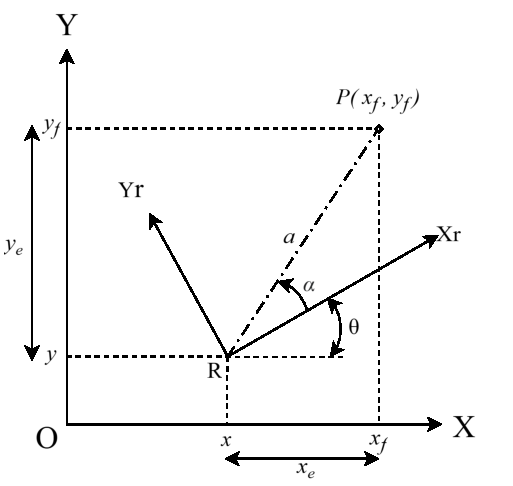
\includegraphics[width=0.9\linewidth]{Pics/error_construccion.pdf}
    \caption{Definición del error}
    \label{fig:error_construccion}
\end{figure}
